%!TEX root = ../my_thesis.tex
\section{Interpretation of the results}
\label{sec:results}

In this thesis, a time-dependent analysis of the decay $\Bz\to \Dmp\pipm$ in order to extract the $\CP$ observables $S_{f}$ and $S_{\bar f}$ was presented. The values obtained are
\begin{align}
 \Sf = \Sfval \pm \Sfstat\stat \pm \Sfsyst \syst\,, \label{eq:result_Sf}\\
\Sfb = \Sfbval \pm \Sfbstat\stat \pm \Sfbsyst \syst\,. \label{eq:result_Sfbar}
\end{align}
The statistical and systematic correlations between \Sf~and \Sfb~are $+60\%$ and $-41\%$, respectively,
and the total correlation is $+44\%$.
These values are in agreement with and more precise than the measurements
from Belle and Babar~\cite{PhysRevD.73.092003,Aubert:2006tw}. A direct comparison is shown in Table~\ref{tab:results_comparison}.
\begin{table}[btp]
	\centering
	\caption{Comparison of the measurements of $S_{f}$ and
	$S_{\bar f}$. The first uncertainty is statistical, the second is systematic.}
	\begin{tabular}{lcc}
		\toprule
		 & $S_{f}$ [\%] & $S_{\bar f}$ [\%] \\
		\midrule
		Belle~\cite{PhysRevD.73.092003} & $+6.8 \pm 2.9 \pm 1.2 $ & $+3.1 \pm 3.0 \pm 1.2 $ \\
                Babar~\cite{Aubert:2006tw} & $-2.3 \pm 4.8 \pm 1.4 $ & $+4.3 \pm 4.8 \pm 1.4 $\\
                LHCb (this analysis)~\cite{Aaij:2018kpq} & $+5.8 \pm 2.0 \pm 1.1 $ & $+3.8 \pm 2.0 \pm 0.7$ \\
		\bottomrule
	\end{tabular}
	\label{tab:results_comparison}
\end{table}

The measurements of $S_{f}$ and $S_{\bar f}$ are interpreted in terms of the angle
$\gamma$ and the strong phase $\delta$, by 
following the definition of $S_{f}$ and $S_{\bar f}$ given in Sec.~\ref{sec:intro}:
\begin{align}
  \label{eq:cpcoeff_theory}
  S_{f}&=-\frac{2r_{D\pi}\sin[\delta-(\gamma+2\beta)]}{1+r_{D\pi}^{2}}, & S_{\bar f}&=\frac{2r_{D\pi}\sin[\delta+(\gamma+2\beta)]}{1+r_{D\pi}^{2}}.
\end{align}
A frequentist method, called PLUGIN and described in Ref.~\cite{Aaij:2016kjh}, is adopted to derive confidence intervals for $\gamma$ and $\delta$
by using external inputs for $\beta$ and $r_{D\pi}$.
Given the observed values $\vec{A}^{\rm obs}=(S_{f}, S_{\bar f})$ and the parameters $\vec{\alpha}=(\gamma,\delta)$, a $\chi^2(\vec{\alpha})$ function
is built as
\begin{equation}
  \label{eq:plugin}
  \chi^2(\vec{\alpha}) = -2\ln\mathcal L(\vec{\alpha}|\vec{A}^{\rm obs}) \hspace{1mm}\propto\hspace{1mm} \left(\vec{A}(\vec{\alpha})-\vec{A}^{\rm obs}\right)^T V^{-1} \left(\vec{A}(\vec{\alpha})-\vec{A}^{\rm obs}\right), 
\end{equation}
where $V$ is the covariance matrix of $S_{f}$ and $S_{\bar f}$. 
The best fit point, $\vec{\alpha}_{\rm min}$, is the one that minimises the expression of Eq.~\ref{eq:plugin}. 
The $p$-value, or 1--CL, is computed for each possible value of each component of $\vec{\alpha}$ ($\gamma$ and $\delta$) as follows:
\begin{enumerate}[noitemsep,topsep=0pt]
  \item a value for a given component of $\vec{\alpha}$ (\eg~$\gamma=\gamma_0$) is chosen, and the associated new minimum $\vec{\alpha}'_{\rm min}(\gamma_0)$ is found;
  \item the corresponding test statistics $\Delta\chi^2=\chi^2(\vec{\alpha}'_{\rm min}(\gamma_0))-\chi^2(\vec{\alpha}_{\rm min})$ is built;
    \item pseudoexperiments are generated to sample values for $\vec{A}$, called $\vec{A}_j$, from $\mathcal L(\vec{\alpha}'_{\rm min}(\gamma_0)|\vec{A})$;
      \item for each $\vec{A}_j$, a new value for the test statistics, $\Delta\chi^2_j$, is computed by replacing $\vec{A}^{\rm obs}\to\vec{A}_j$ 
        in Eq.~\ref{eq:plugin}, and
        by taking the difference between the minimised values of $\chi^2$ with respect to $\vec{\alpha}$, once with $\gamma$ as free
        parameter, and once with $\gamma=\gamma_0$;
        \item the $p$-value is computed as the fraction of pseudoexperiments for which $\Delta\chi^2<\Delta\chi^2_j$.
\end{enumerate}
In all the minimisation steps described above, the values $\beta=(22.2 \pm 0.7)^{\circ}$~\cite{HFAG} and
$r_{D\pi}=(1.82 \pm 0.12 \pm 0.36(\textrm{\small{SU(3)}}))\%$ are used as external Gaussian constraints. 
The latter is calculated from the branching fraction
of $\Bz \to \Dsp \pim$ decays, assuming SU(3) symmetry, following the relation of Refs.~\cite{Das:2010be,Aubert:2008zi}:
\begin{equation}
\label{eq:rdpi_1}
r_{D\pi}= \tan \theta_c  \frac{f_{D}}{f_{D_s}}\sqrt{\frac{\mathcal{B}(\Bz \to \Dsp \pim)}{\mathcal{B}(\Bz \to \Dm \pip)}},
\end{equation}
where $ \tan \theta_c= 0.23101 \pm 0.00032$~\cite{CKMfitter2015} is the tangent of the Cabibbo angle,
$\frac{f_{D_s}}{f_{D}}= 1.173 \pm 0.003$~\cite{Aoki:2016frl,Bazavov:2014wgs,Carrasco:2014poa} is the ratio of decay constants,
$\mathcal{B}(\Bz \to \Dsp \pim)=(2.16 \pm 0.26)\times10^{-5}$~\cite{PDG} and $\mathcal{B}(\Bz \to \Dm \pip)=(2.52 \pm 0.13)\times10^{-3}$~\cite{PDG}.
 An additional $20\%$ relative error is added on $r_{D\pi}$ to account for
uncertainties due to  possible non-factorizable SU(3)-breaking effects, as reported in Ref.~\cite{DeBruyn:2012jp}.

The angle $\gamma$ is determined to be in the interval \gammaCL~and $\delta$ to be in the interval \deltaCL, both at the $68\%$ CL. These intervals are illustrated in Fig.~\ref{fig:gammacombo}.
In Fig.~\ref{fig:gammaCombo2D}, contours are shown in the two-dimensional plane ($\gamma$, $\delta$). 

In addition to $\gamma$ and $\delta$, the interval
of $|\sin(2\beta +\gamma)|$ is determined as well. This quantity does not rely on any external input for $\beta$, and it is thus experimentally
cleaner. This interval is found
to be \magSinTwoBplusGCL~at the $68\%$ CL as shown in Fig.~\ref{fig:gammaCombo_sin2b+g}.
The absolute value of $\sin(2\beta +\gamma)$ is considered because the decay-time fit cannot resolve the ambiguity on the sign, \ie~the 
same $p$-value is found for $2\beta +\gamma$ and $-(2\beta +\gamma)$. 

The intervals for $\gamma$, $\delta$ and $|\sin(2\beta +\gamma)|$ are also determined by assuming a SU(3)-breaking uncertainty of $0\%$, $20\%$ and $100\%$
on the value of $r_{D\pi}$. These are presented in
Figs.~\ref{fig:SU3_gammaCombo_g_d} and~\ref{fig:SU3_gammaCombo_sin2b+g}.

\begin{figure}[t]
	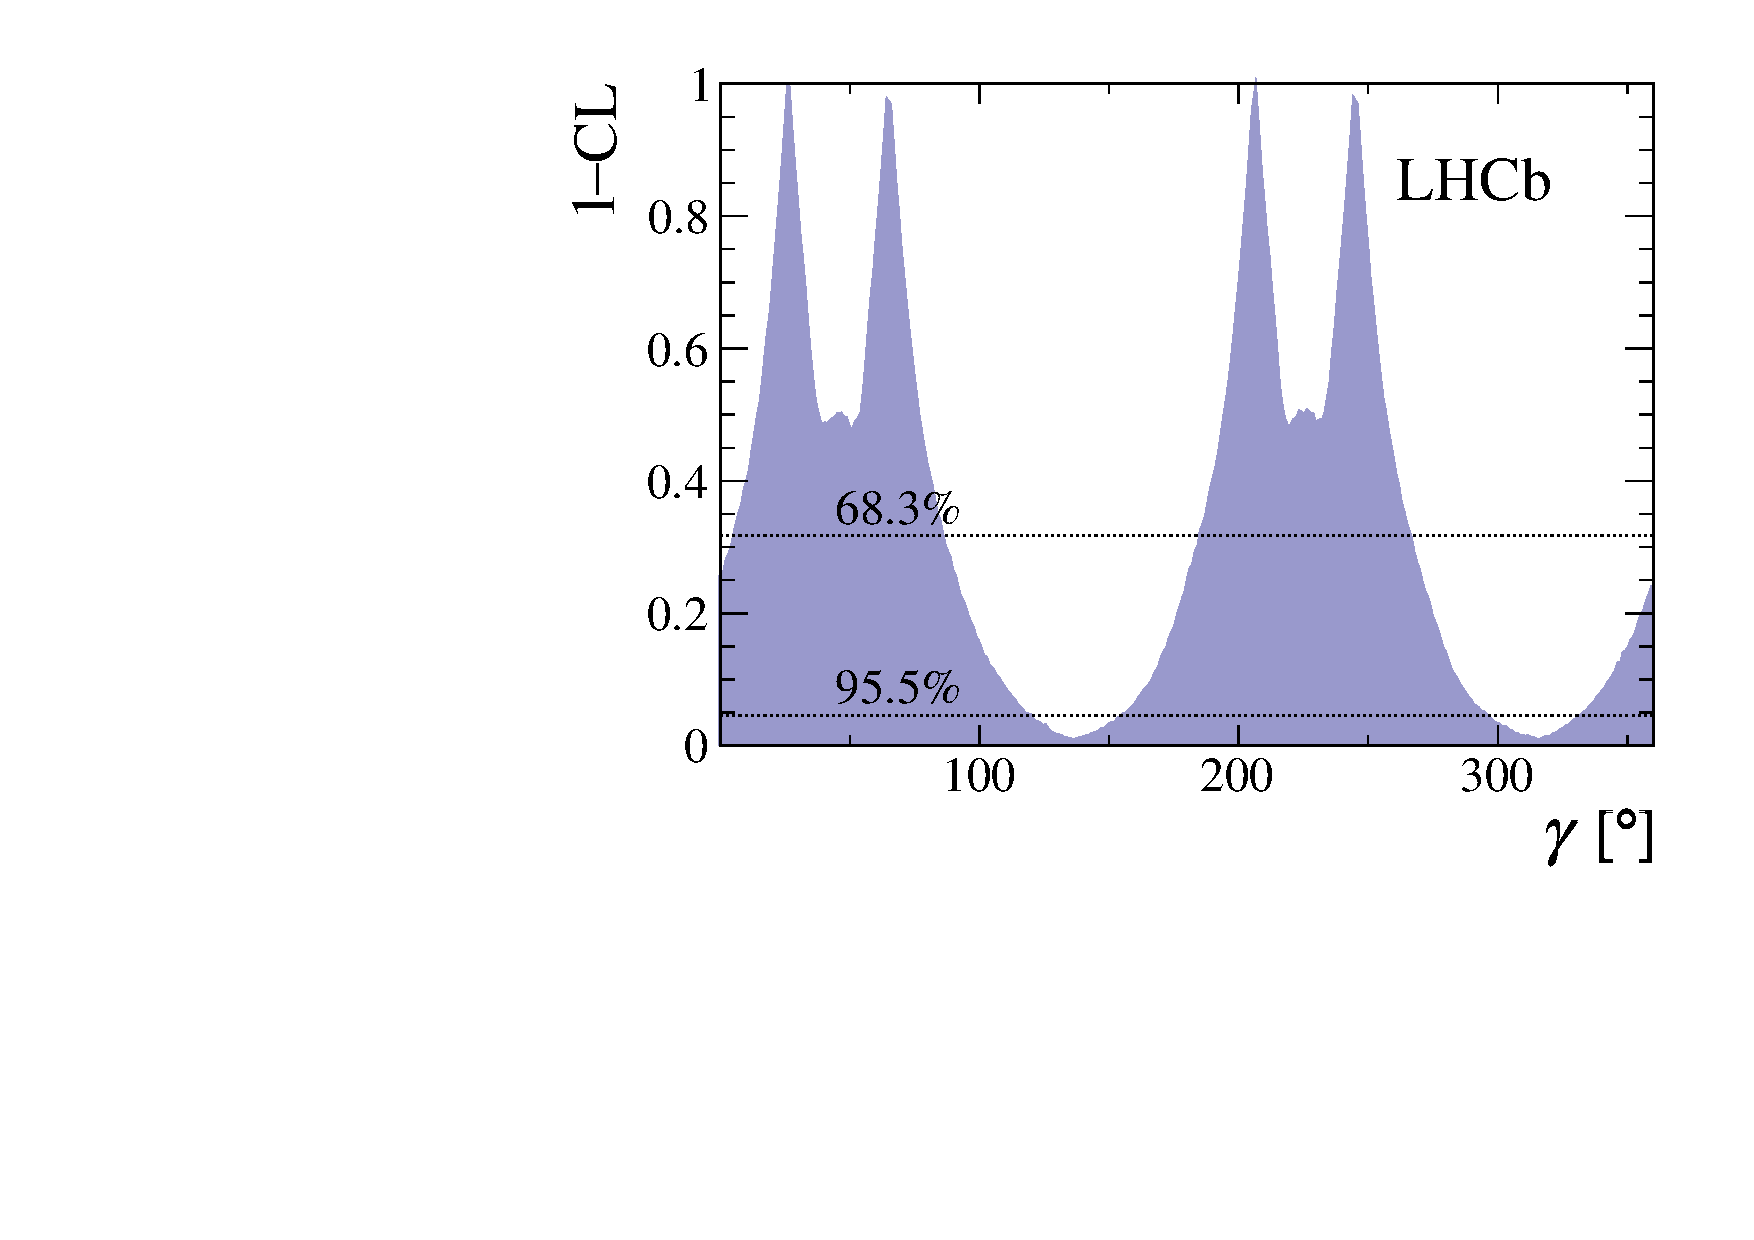
\includegraphics[width=0.49\textwidth]{07Results/figs/gammacombo_bd2dmpip_g.pdf}
	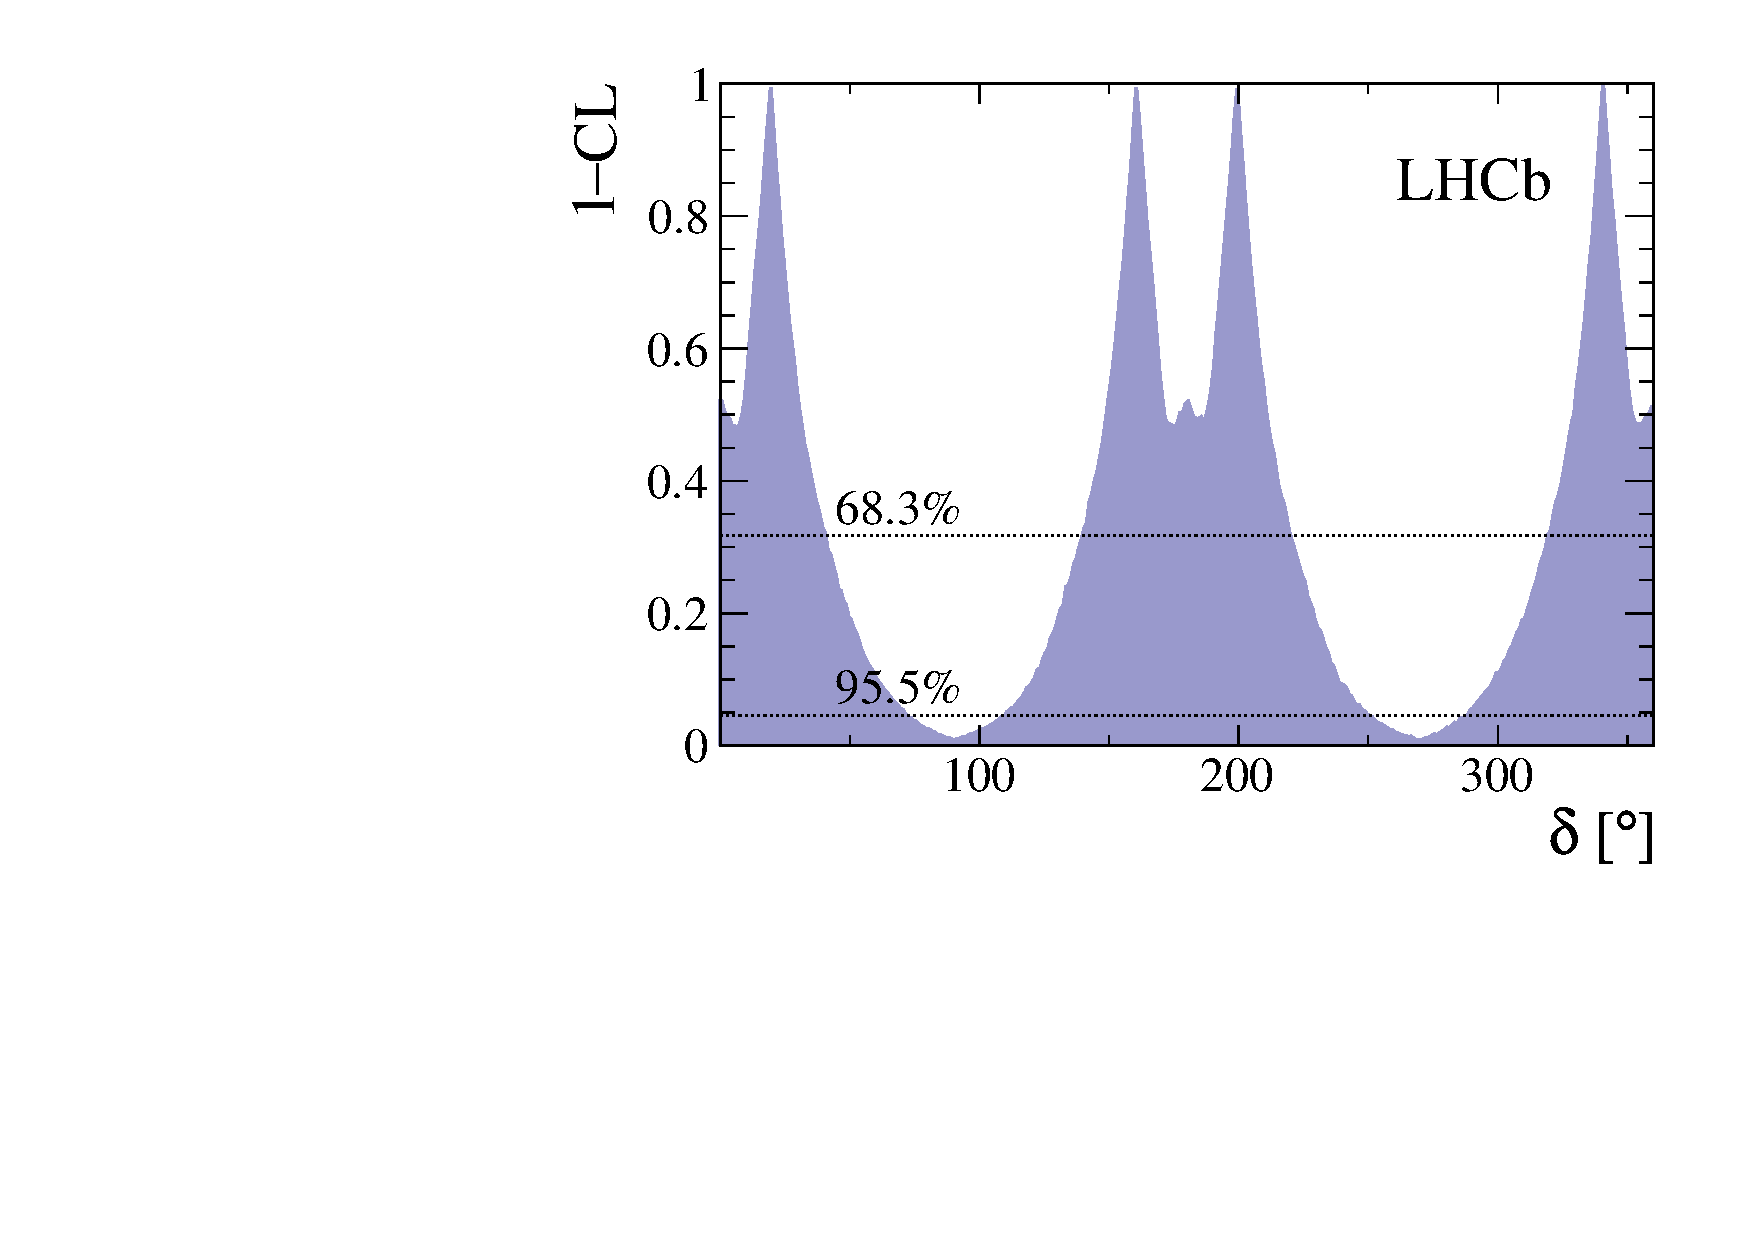
\includegraphics[width=0.49\textwidth]{07Results/figs/gammacombo_bd2dmpip_d_dmpi.pdf}
	\vspace{-2mm}
        \caption{$p$--value, or 1--CL, as a function of $\gamma$ (left) and $\delta$ (right) obtained using the measured values of $S_{f}$
	and $S_{\bar f}$.}
	\label{fig:gammacombo}
\end{figure}

\begin{figure}[t]
\centering
	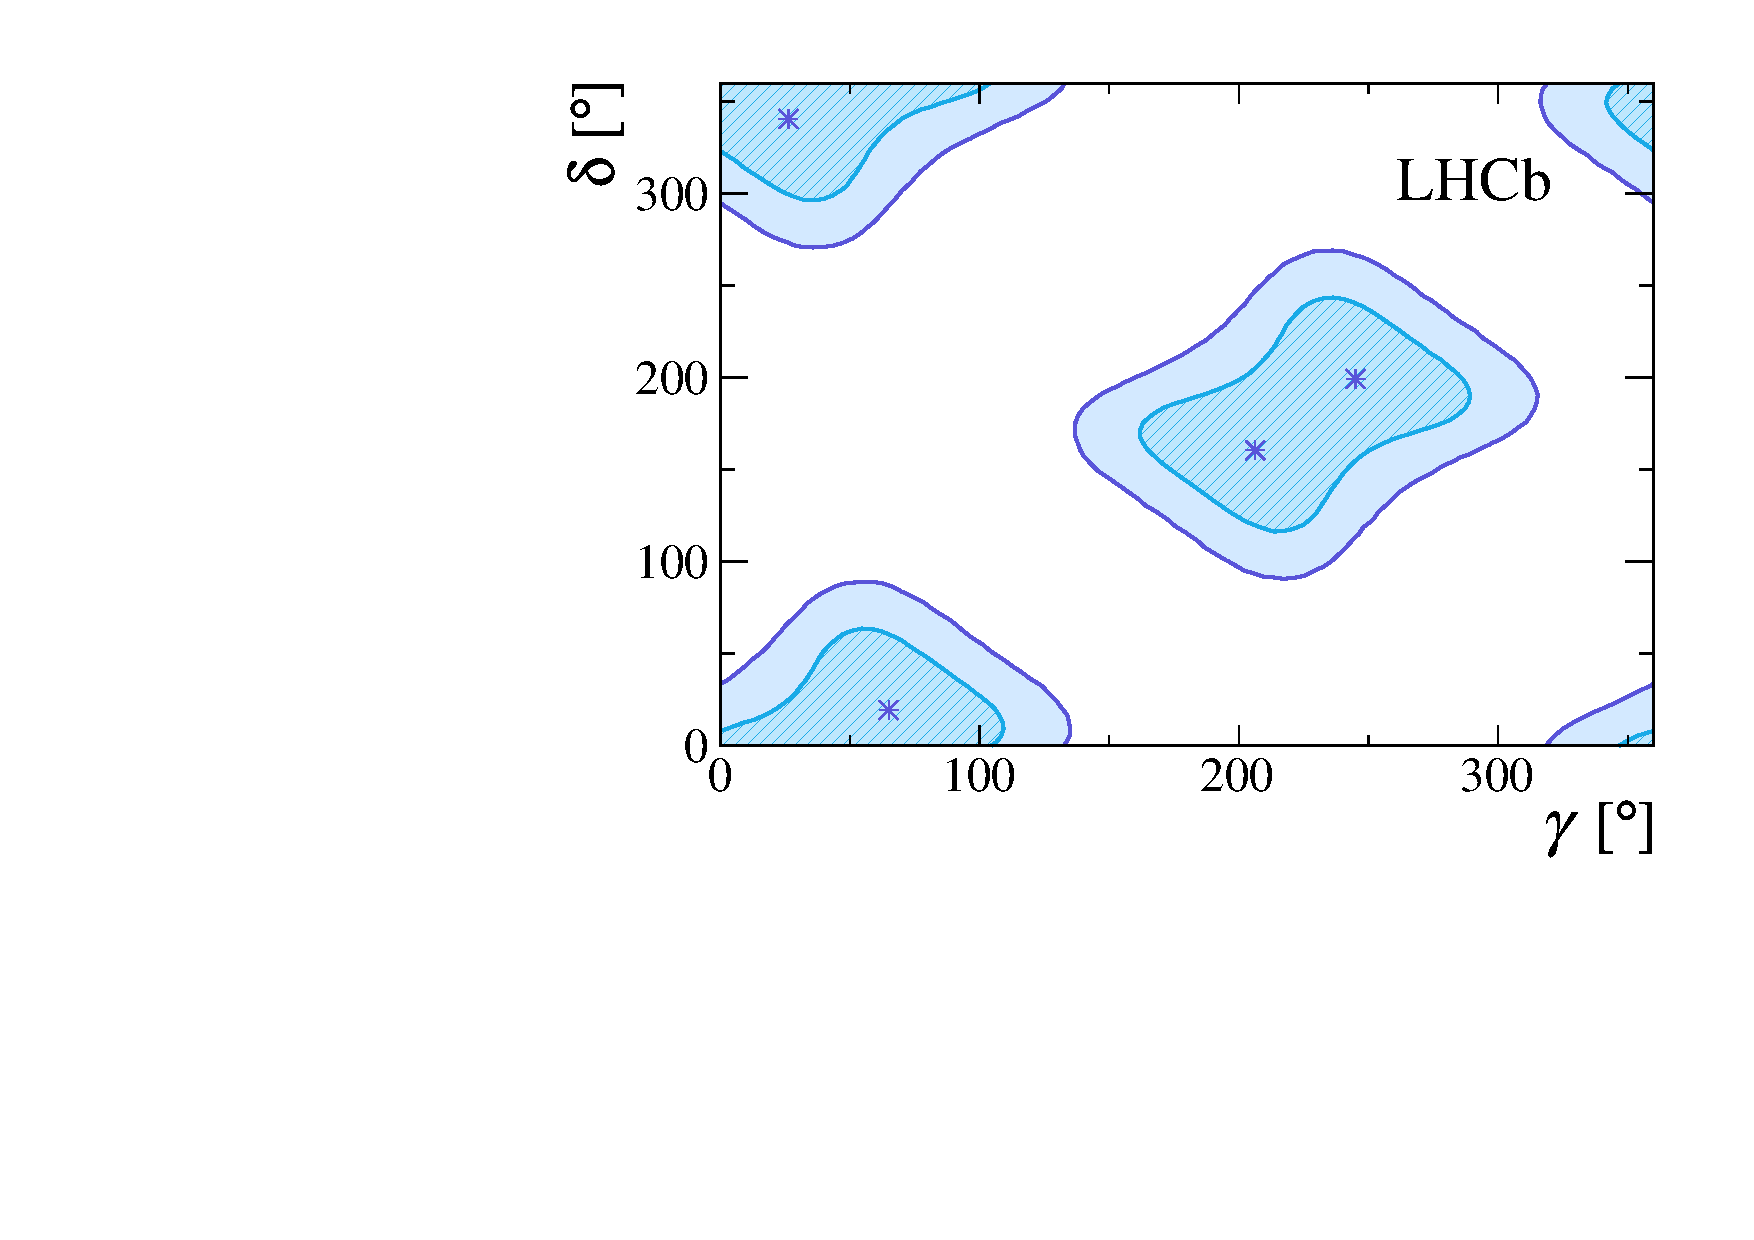
\includegraphics[width=0.6\textwidth]{07Results/figs/gamma_delta_lhcb.pdf}
	\vspace{-2mm}
        \caption{Contours in the two-dimensional plane ($\gamma$, $\delta$) obtained using the measured values of $S_{f}$
	and $S_{\bar f}$. The crosses indicates the preferred values (1--CL=1). The blue hatched (solid) areas correspond to $39\%$ ($87\%$) confidence level.}
	\label{fig:gammaCombo2D}
\end{figure}

\begin{figure}[t]
\centering
	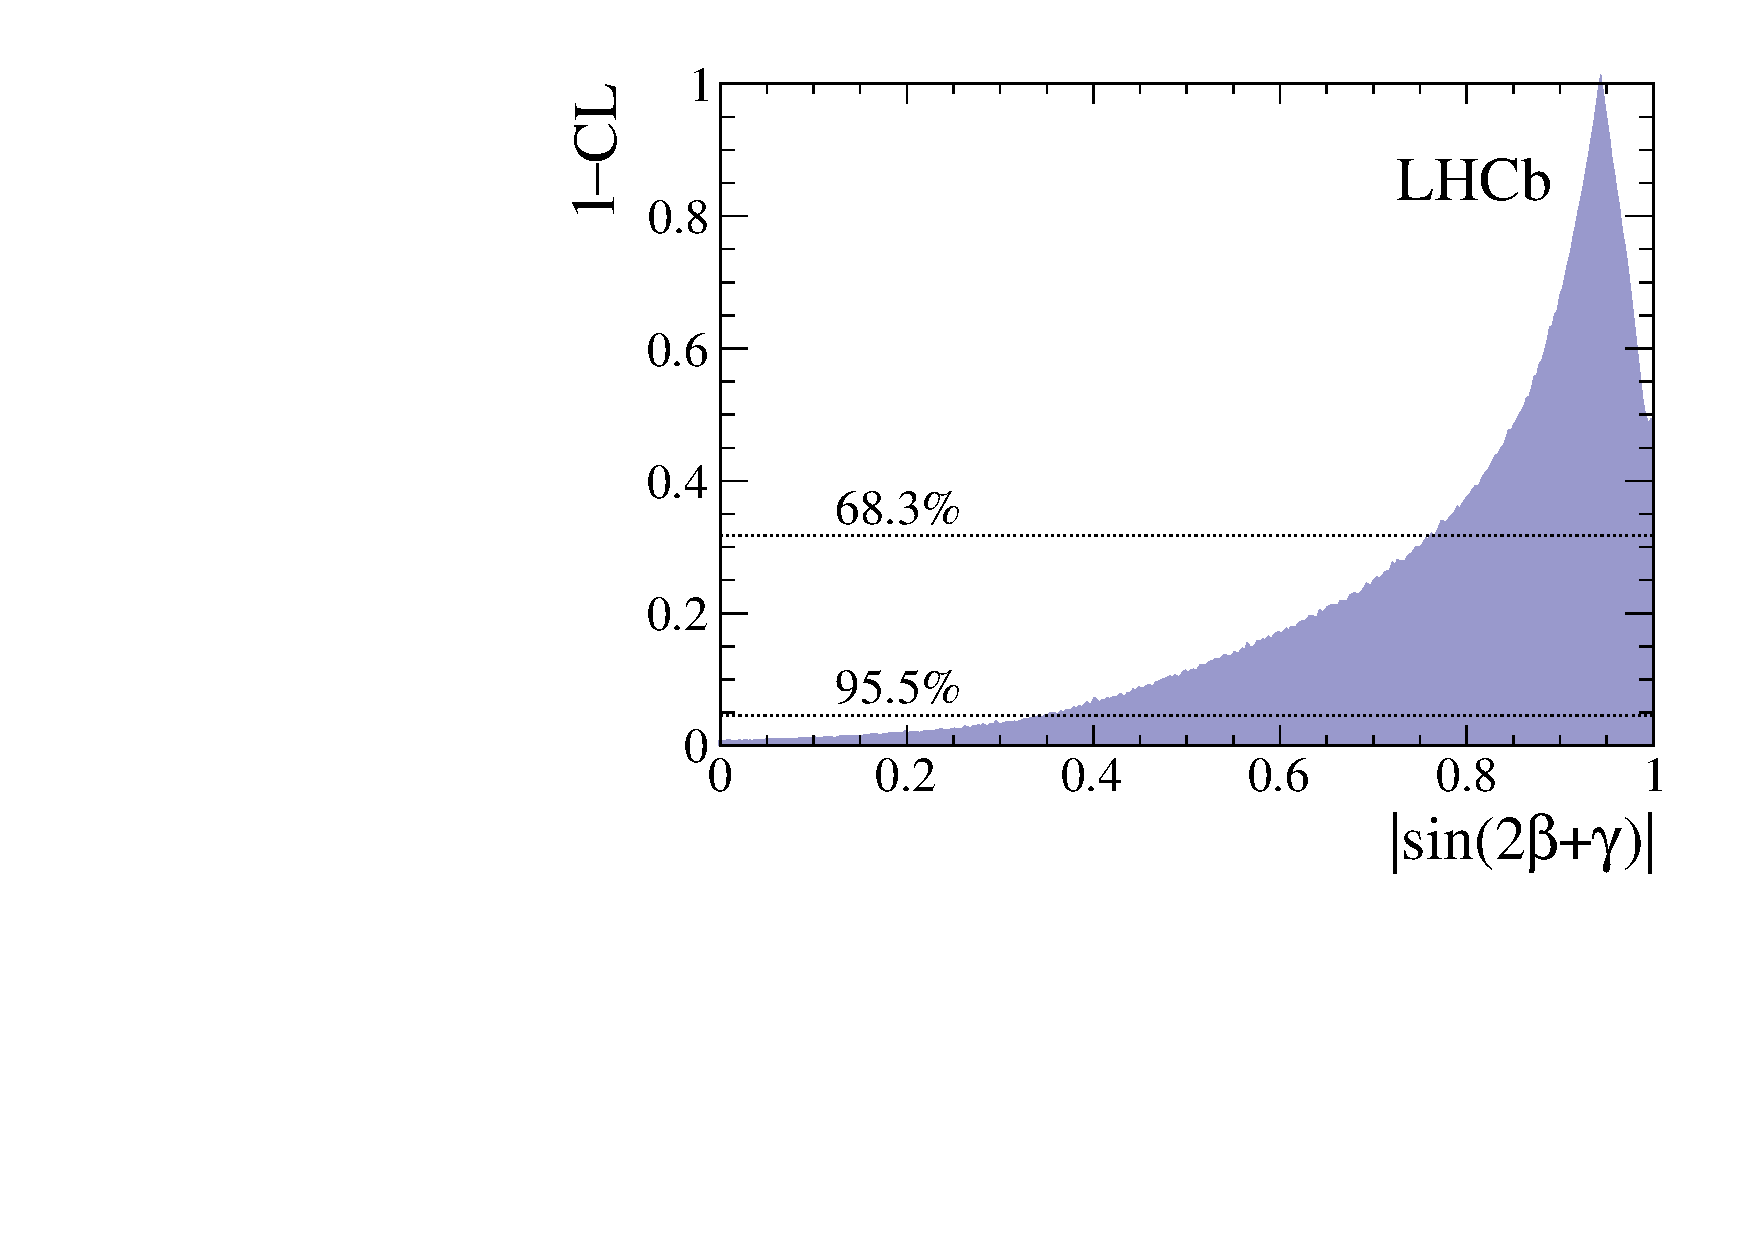
\includegraphics[width=0.6\textwidth]{07Results/figs/gammacombo_sin_2b_g.pdf}
	\vspace{-2mm}
        \caption{$p$--value, or 1--CL, as a function of $\left|\sin\left(2\beta+\gamma\right)\right|$ using the measured values of $S_{f}$ and $S_{\bar f}$.}
	\label{fig:gammaCombo_sin2b+g}
\end{figure}

\begin{figure}[t]
\centering
	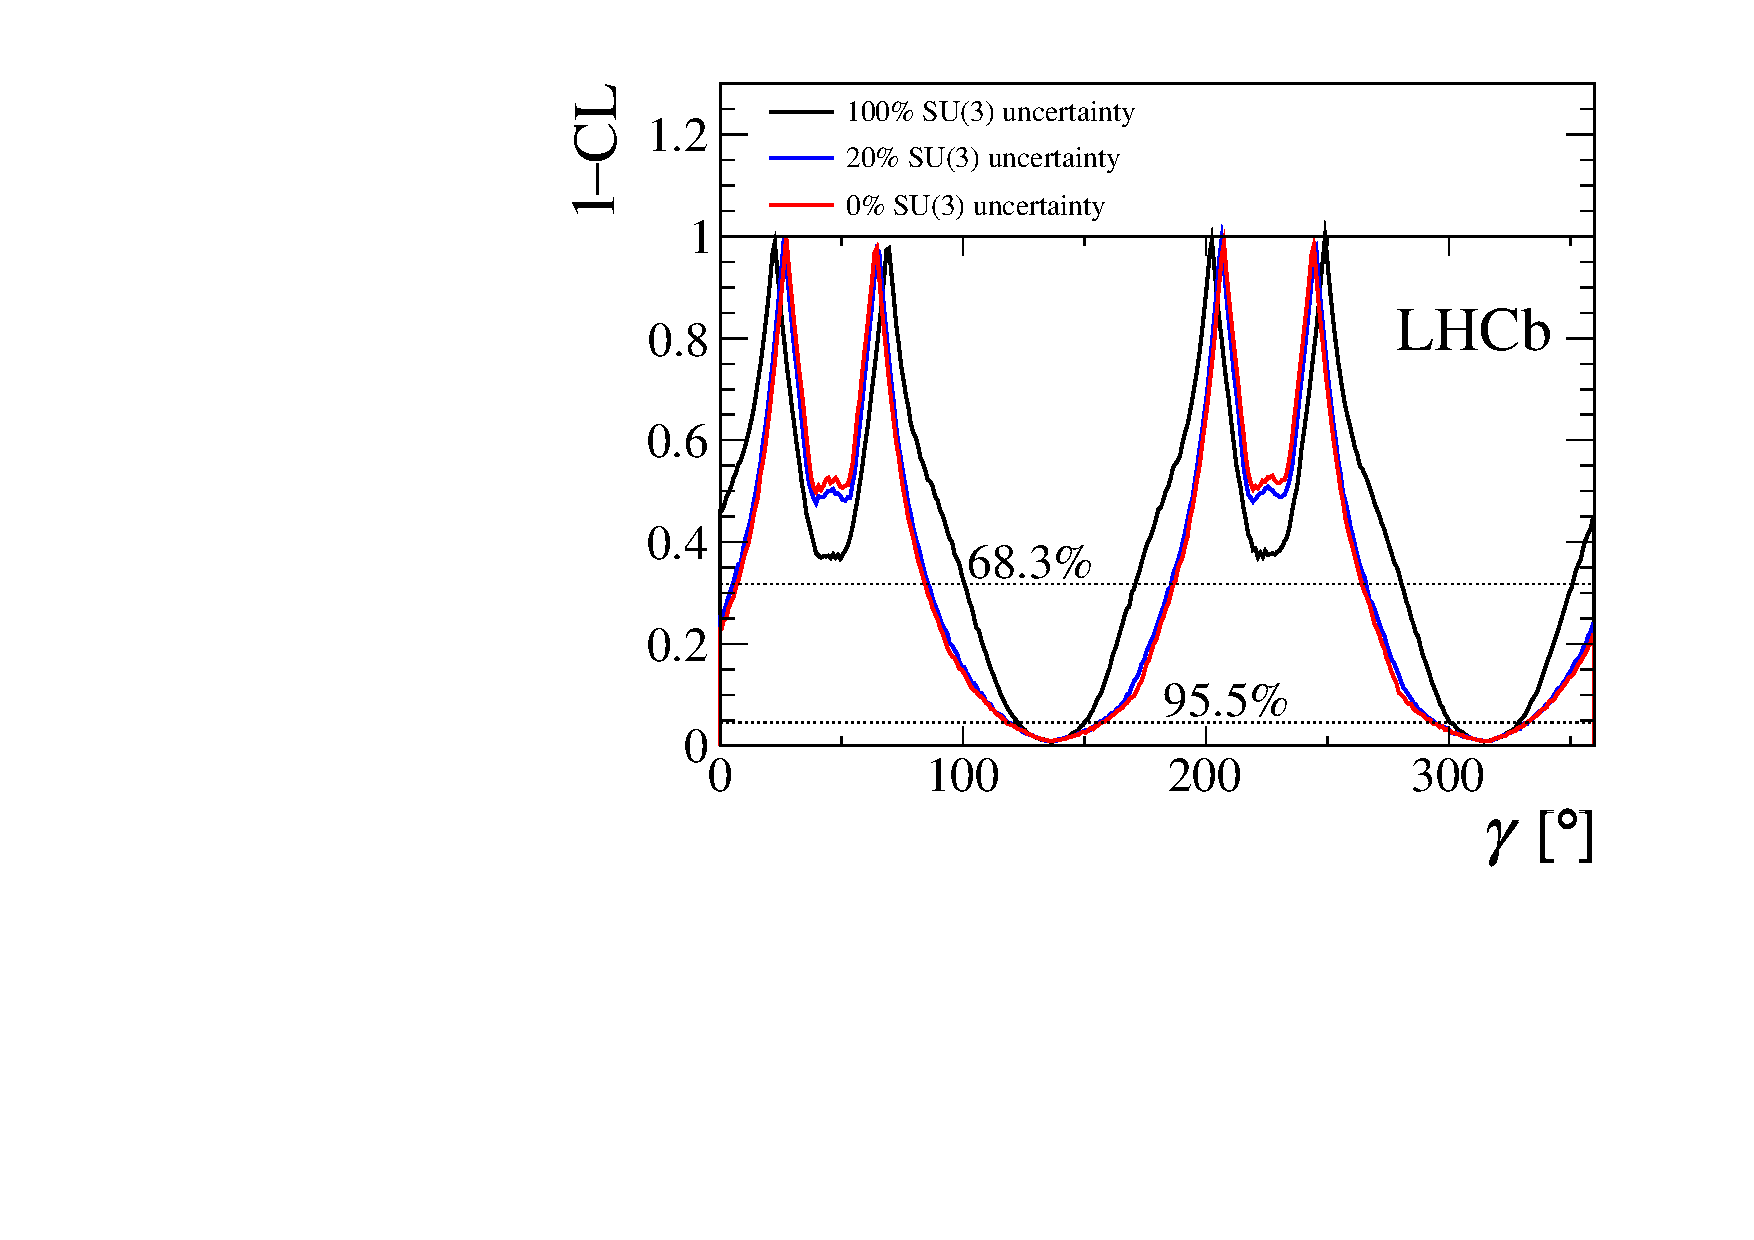
\includegraphics[width=0.49\textwidth]{07Results/figs/su3_scan_bd2dpi_g.pdf}
	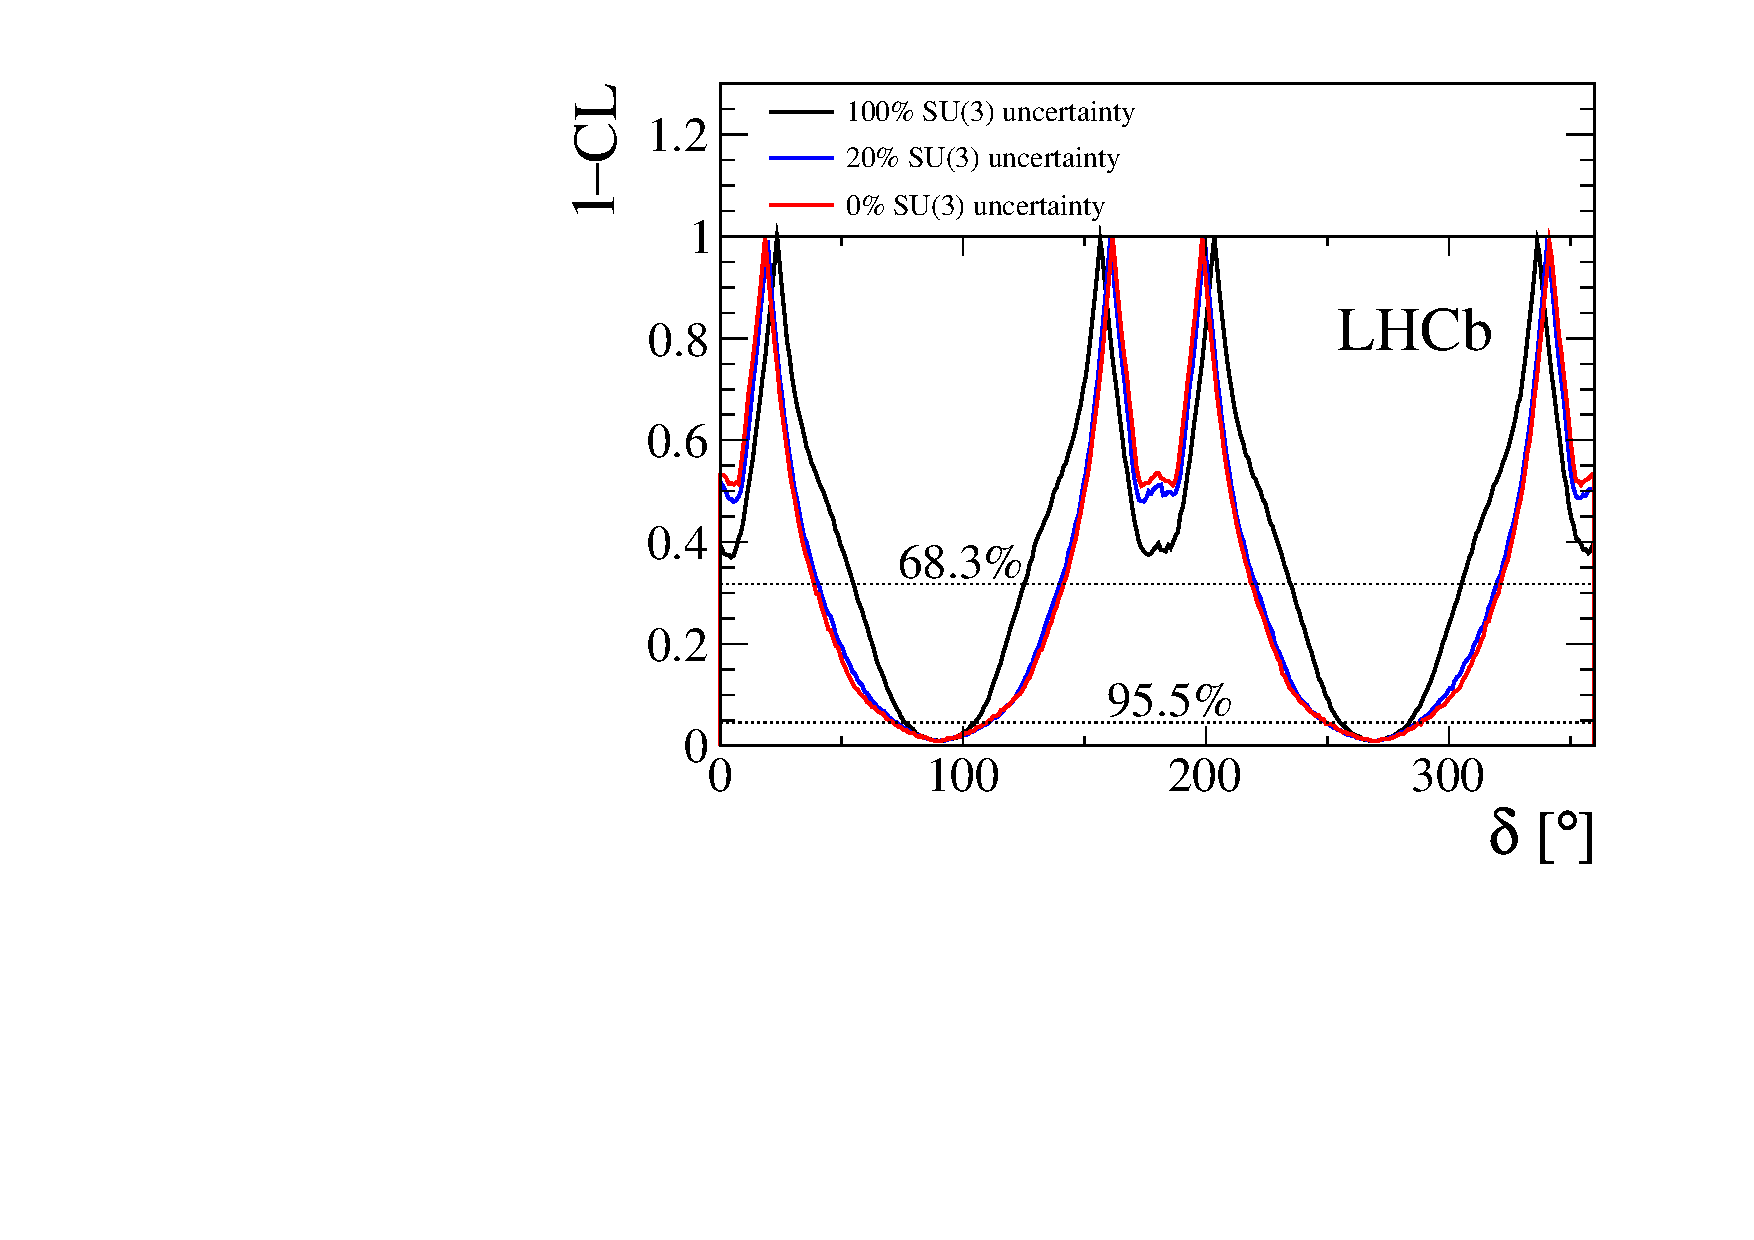
\includegraphics[width=0.49\textwidth]{07Results/figs/su3_scan_bd2dpi_d.pdf}
	\vspace{-2mm}
        \caption{$p$--value, or 1--CL, as a function of (left) $\gamma$ and (right) $\delta$ for assumptions of \SI{0}{\percent}, \SI{20}{\percent} and \SI{100}{\percent}
  for the SU(3) uncertainty on the parameter $r_{D\pi}$.}
	\label{fig:SU3_gammaCombo_g_d}
\end{figure}

\begin{figure}[t]
\centering
	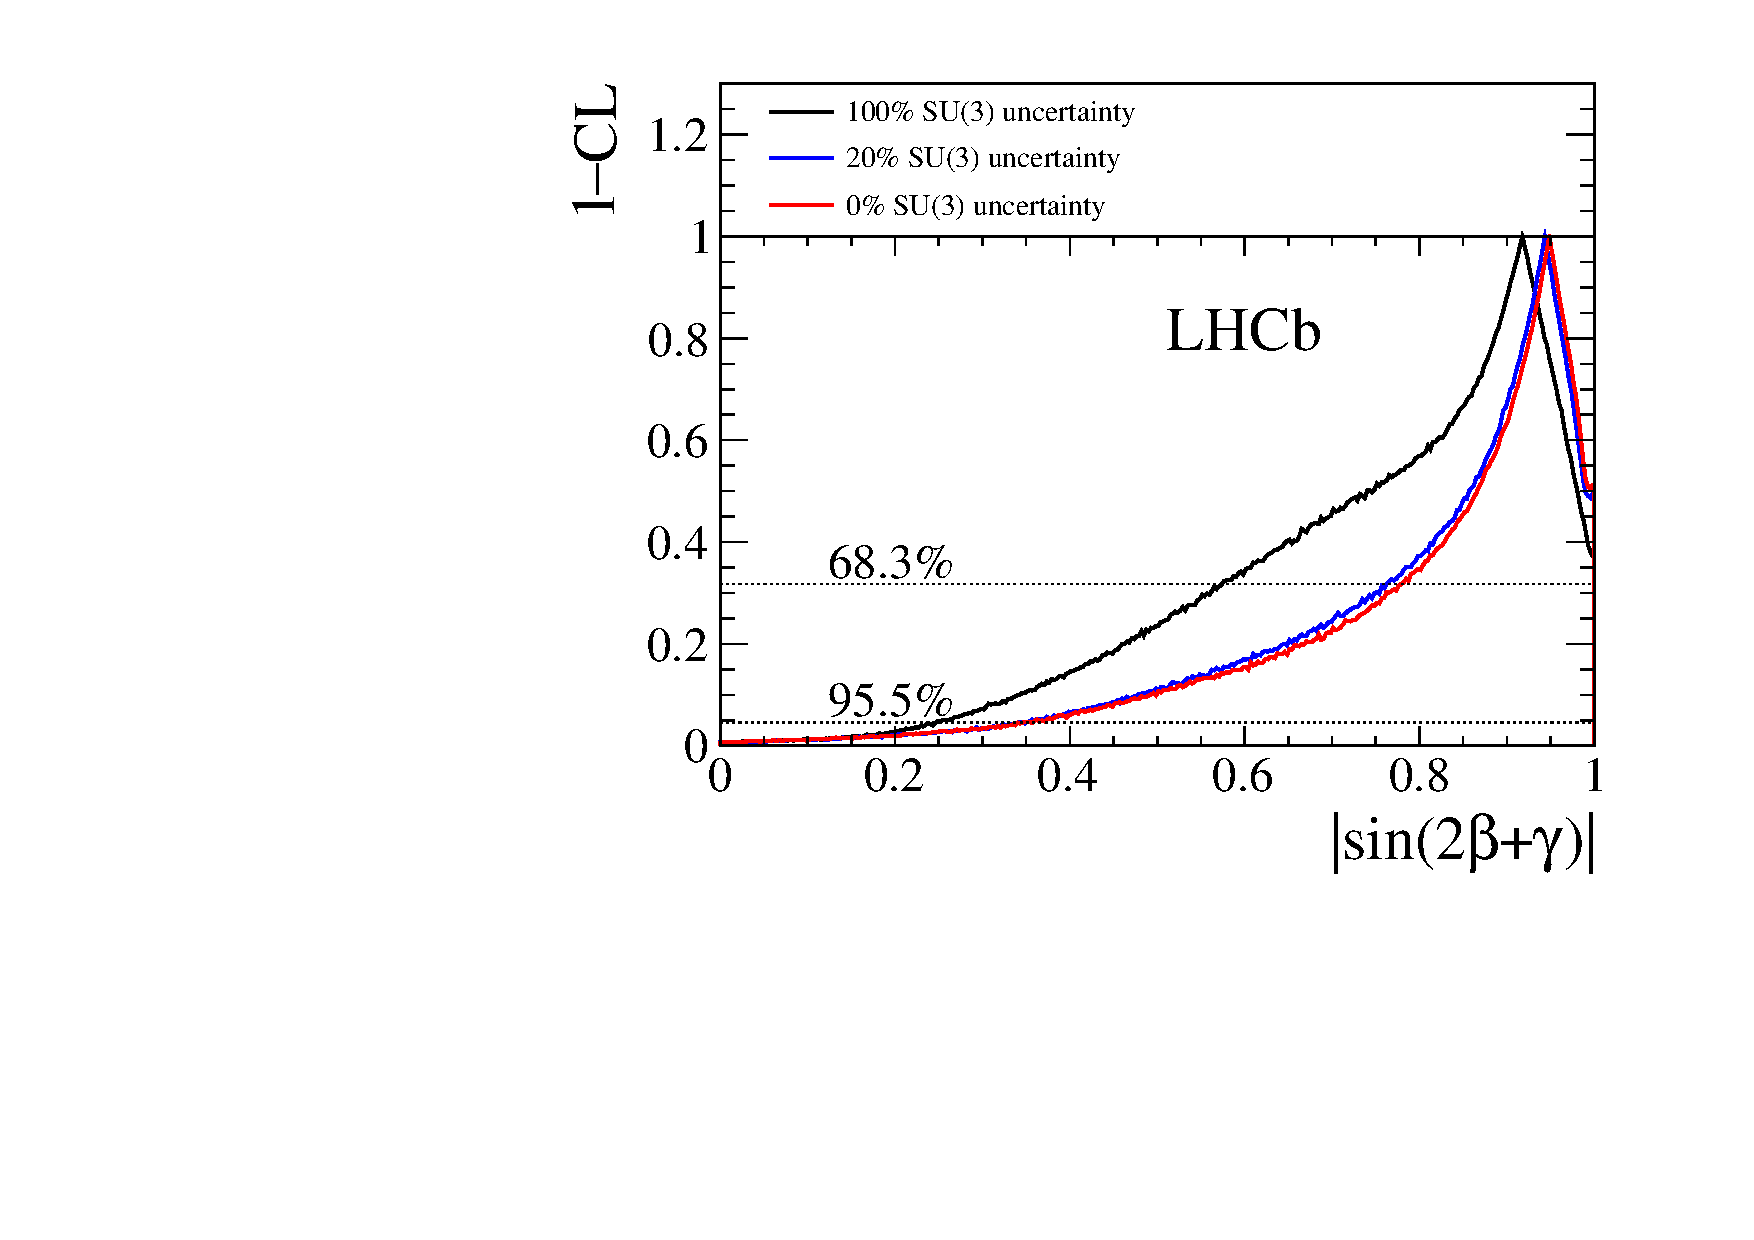
\includegraphics[width=0.6\textwidth]{07Results/figs/su3_scan_sin2b_plus_gamma.pdf}
	\vspace{-2mm}
        \caption{1--CL as a function of $|\sin(2\beta+\gamma)|$ for assumptions of \SI{0}{\percent}, \SI{20}{\percent} and \SI{100}{\percent}
  for the SU(3) uncertainty on the parameter $r_{D\pi}$.}
	\label{fig:SU3_gammaCombo_sin2b+g}
\end{figure}

%%%%%%%%%%%%%%%%%%%%%%%%%%%%%%%%%%%%%%%%%%%%%%%%%%%%%%%%%

\section{Summary and perspectives}
\label{sec:outlook}

The $\Bz\to\Dmp\pipm$ analysis presented in this thesis was performed on the full LHCb Run~1 (2011--2012) dataset,
corresponding to an integrated luminosity of $3~\rm fb^{-1}$.

As can be seen from Eqs.~\ref{eq:result_Sf} and~\ref{eq:result_Sfbar}, 
the dominant contribution in the error budget of $S_f$ and $S_{\bar f}$ is the statistical uncertainty.
For this reason, the precision of the measurement can be easily improved by using a larger data sample.

The statistics expected to be collected during Run 2 (2015--2018) is $\sim 6~\rm fb^{-1}$, with a luminosity of $4\times 10^{32}~\rm cm^{-2}s^{-1}$.
The centre-of-mass energy during Run 2 ($13~\rm TeV$) is about twice the Run 1 value; for this reason, the $\Bz$ production cross-section
is also increased approximately by a factor two compared to Run 1. So, the increase in the number of reconstructed $\Bz\to\Dmp\pipm$ decays in Run 2 compared
to Run 1 is about $\sim 2\times \frac{6}{3} = 4$, which corresponds to a factor $\sim \sqrt{4}=2$ of decrease in statistical uncertainty.
 
After Run 2, a two-year shutdown (2019--2020) will allow 
a major upgrade of several LHCb detectors to take place. Particularly relevant for the $\Bz\to\Dmp\pipm$ analysis
are the VELO upgrade~\cite{LHCb-TDR-013}, which will imply an improvement of hit efficiency and IP resolution thanks to the pixel geometry,
the Upstream Tracker~\cite{Collaboration:1647400} (replacing the TT), which will improve the particle acceptance,  
and the scintillating
fibre tracker~\cite{Collaboration:1647400} (replacing IT and OT), which is designed to cope with the expected higher occupancy due to the higher luminosity.
Moreover, the L0 trigger will be removed, and a $40$~MHz readout electronics will be installed; a fully software-implemented trigger will thus be adopted.
According to Ref.~\cite{LHCb-PUB-2014-040}, the resulting trigger efficiencies for fully hadronic decays as $\Bz\to\Dmp\pipm$ is expected to
increase by a factor $\sim 2$ compared to Run 1.
The LHC will restart in 2021 with an increased luminosity of $2\times 10^{33}~\rm cm^{-2}s^{-1}$,
and $pp$ collisions at a centre-of-mass energy of $14~\rm TeV$ will be delivered during Run 3 (2021--2023) and Run 4 (2026--2029).
At the end of Run 4, the total amount of data collected with the upgraded detector is expected to reach $\sim 50~\rm fb^{-1}$. 
The expected increase in the number of reconstructed $\Bz\to\Dmp\pipm$ decays
in Runs 3 and 4 is about $\sim 2\times 2\times \frac{50}{3}\sim 70$, which corresponds to a factor $\sim\sqrt{70}\sim 8$ of decrease in statistical uncertainty
compared to the Run 1 result.

Finally, a second upgrade of LHCb is under discussion, which would allow the experiment
to operate at a luminosity of $1-2\times 10^{34}~\rm cm^{-2}s^{-1}$ starting in 2031~\cite{Upgrade2}.
The expected $pp$ collision statistics that will be collected in this high-luminosity scenario corresponds to $\sim 300~\rm fb^{-1}$.
Given the same centre-of-mass energy of $14~\rm TeV$, the increase in the number of $\Bz\to\Dmp\pipm$ decays will be about $\sim 2\times2\times \frac{300}{3}\sim 400$, corresponding to a reduction of the Run 1 statistical uncertainty by a factor $\sim\sqrt{400}\sim 20$.

These extrapolations are made by assuming the same tagging power as obtained on Run 1 data; future developments of flavour tagging algorithms
are thus crucial to further improve these projections. As described in Sec.~\ref{sec:tagging:OSePerf2}, the performance of OS taggers on Run~2 data is
compatible with, and not worse than, the one obtained on Run 1 data thanks to the reoptimisation campaign on Run~2 data, while the tagging power
of the \SSpi~and \SSp~taggers is increased. Preliminary studies on simulated samples showed that both SS taggers and Run 2-optimised OS taggers
have similar performances in Run 3 as the ones of Run 2; further improvements can be achieved by tuning these taggers specifically on Run 3 (and beyond) conditions. In parallel, a new approach, called \emph{inclusive tagger}, is under development. This algorithm, consisting of a deep neural network, exploits
all tracks and vertices reconstructed in the events in order to provide a tagging decision and a mistag estimate. 
Preliminary results on Run 1 $B^+\to J/\psi K^+$ data indicate a tagging power of the order of $~\sim 7-8\%$, which would represent a relative
increase of $\sim 40-60\%$ compared to the combination of the standard OS and SS taggers.
 
Concerning the systematic uncertainties on $S_f$ and $S_{\bar f}$, the external constraint on $\Delta m$, which is the dominant contribution to the systematic error budget, 
will also benefit from the high
statistics collected by LHCb, since the world-leading measurement of this parameter is already obtained by the LHCb collaboration 
from semileptonic \Bz~decays~\cite{LHCB-PAPER-2015-031}, and this result will be updated with new data.
In addition to $\Delta m$, other sources of systematic uncertainty ($\Delta\Gamma$, decay-time resolution \dots) are expected to be reduced thanks to the increased statistics foreseen for the next decades.

The precision on the values of $\gamma$ and $\delta$ extracted from the measured values for $S_f$ and $S_{\bar f}$ will benefit from the increased
knowledge on $\beta$ and $r_{D\pi}$. The $\beta$ angle will be measured with unprecedent precision also thanks to the Belle II experiment~\cite{Aushev:2010bq,Abe:2010gxa}, which will start its operations between 2018 and 2019. 
The precision on the $r_{D\pi}$ parameter will increase thanks to the improvement in the measurements
of the $\Bz \to \Dsp \pim$ and $\Bz \to \Dm \pip$ branching ratios, according to Eq.~\ref{eq:rdpi_1}. Moreover, if the $\Bs\to D^+ K^-$ decay will be observed, an independent
estimation of $r_{D\pi}$ will be available by following the relation
\begin{equation}
  \label{eq:rdpi_2}
  r_{D\pi} = \frac{f_{\pi}}{f_{K}}\sqrt{\frac{\mathcal{B}(\Bs \to D^+ K^-)}{\mathcal{B}(\Bz \to \Dm \pip)}}, 
\end{equation}
where SU(3) symmetry is assumed as for Eq.~\ref{eq:rdpi_1} and $\frac{f_{\pi}}{f_{K}}=1.1956(10)^{+26}_{-18}$~\cite{Bazavov:2014wgs}.
A search for $\Bs\to D^+ K^-$ with Run 1 data gave a null result~\cite{matthieu}.

The value of $\gamma$ that will be extracted with future time-dependent analyses of $\Bz\to\Dmp\pipm$ decays, and similarly of $\Bs\to D_{s}^{\mp} K^{\pm}$ decays,
will be one of the inputs for the global combination of direct measurements performed by LHCb. The current sensitivity, which is of the order
of $\sim 5-6^\degree$~\cite{Aaij:2016kjh}, is expected to go down at the level of $\sim 0.4^\degree$ with $\sim 300~\rm fb^{-1}$ of collected 
data~\cite{CERN-LHCC-2017-003}. 
This sensitivity will allow to test the expected relationship between $\gamma$ and the \CP~coefficients 
given by Eq.~\ref{eq:cpcoeff_theory}, which is affected by small theoretical uncertainties,  
and to compare these direct measurements of $\gamma$ with the indirect determination from other CKM parameters: a discrepancy in any of these tests
will be a clear signature of new physics beyond the SM.
